% % Section and Frames
% \section{Framework Implementation Overview}
% \label{framework_implementation_overview_section}
% 
% % Section title frame
% \sectiontitleframe{Framework Implementation Overview}

\begin{frame}[fragile]{Framework Overview}
    \frametitle{Framework Overview}

    \begin{lstlisting}[caption={Example Usage of the Image Preprocessing Framework.}, label=lst:frameworkusage, basicstyle=\scriptsize\ttfamily]
# Initialize the image preprocessor
preprocessor = (*@\class{ImagePreprocessor}@*)()

# Define the preprocessing pipeline
pipeline = [
    (*@\class{AdaptiveHistogramEqualizer}@*)(clip_limit=4.0, tile_gridsize=[4,4]),
    (*@\class{ShapeResizer}@*)(desired_shape=[2000, 2000], method='bilinear')
    (*@\class{MeanNormalizer}@*)()
]

# Set and process the pipeline
preprocessor.set_pipe(pipeline)
processed_dataset = preprocessor.process(image_dataset)
    \end{lstlisting}
\end{frame}

\begin{frame}{Framework Architecture - UML Diagram}
    \frametitle{Framework Architecture}
    % The following UML (Unified Modeling Language) diagram provides a visual representation of the Image Preprocessing Framework's architecture, illustrating the interplay between various components.
    \begin{figure}
        \center
        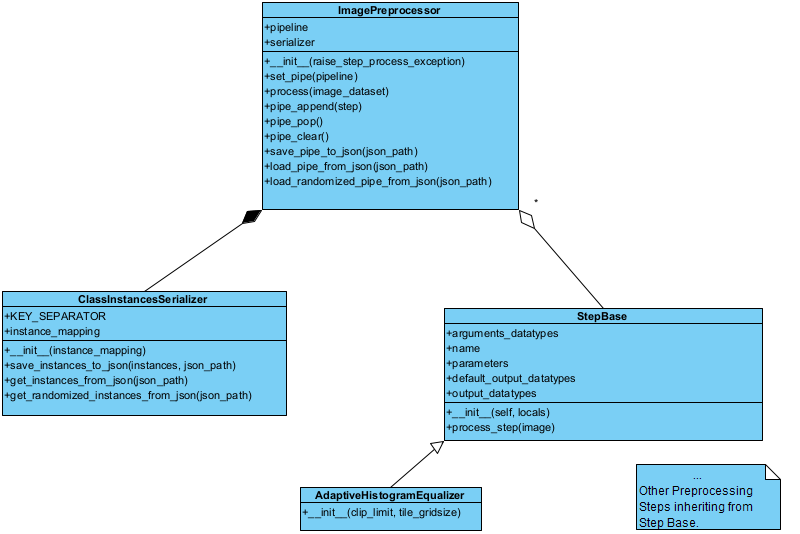
\includegraphics[width=0.8\textwidth]{figures/image_preprocessing_uml.png}
        \caption{UML Diagram of the Image Preprocessing Framework.}
        \label{fig:uml_diagram}
    \end{figure}
\end{frame}

% \begin{frame}{Key Components and Interactions}
%     \frametitle{Key Components and Interactions}
%     The UML diagram highlights the critical components of the framework:
%     \begin{itemize}
%         \item \textbf{ImagePreprocessor:} The core component managing the preprocessing pipeline.
%         \item \textbf{StepBase:} An abstract base class for all preprocessing steps.
%         \item \textbf{Concrete Steps:} Specific implementations of preprocessing tasks (e.g., shape resizer, mean normalizer).
%         \item \textbf{ClassInstancesSerializer:} Manages the serialization and deserialization of the pipeline.
%     \end{itemize}
%     Together, these elements enable a versatile and effective image preprocessing workflow.
% \end{frame}
